\chapter{Introduction}

With the emergence of new sequencing systems genomic data is being generated at an unprecedented rate.Almost two decades back \textbf{The Human Genome Project} took 13 years and over 3 billion dollars to sequence the entire human genome whereas the same information can be sequenced today in under an hour for 1000 dollars.This rapid improvement in sequencing genomic data has improved the availability of high resolution genomics data and has helped researchers in answering a wide range of biological questions.

An important field in biological research where genomic data is extensively used is comparative genomics.It involves comparing genomic information between different species to understand their similarity.A genome of an organism consists of its complete set of DNA in the form of a series of genes where every gene is a sequence that is responsible for one or more traits in that organism.Comparing genomic sequences between two different organisms can help researchers in understating their evolutionary relationship as similar sequences can often mean that the genes have the same function.Such similar sequences are referred to as homologous sequences and they indicate shared ancestry.As organism evolve overtime and diversify into different species they retain parts of their DNA from their common ancestor.The study of these conserved homologous regions is called \textbf{Synteny}. 

While a huge part of comparing large scale genomic sequences is purely computational and thus can be automated human judgement is still vital in syteny analysis.Visual data exploration for example can help researchers in easily identifying similarities among large scale genomes as humans are intuitively good at picking out patterns in pictures and visuals.Synteny visualization commonly involves visualizing genomes at the whole genome level or the individual chromosome level and representing similar genes either by connected links or similar colored regions.Syntenic data analysis can often be an iterative process where researchers visualize computational results multiple times under various parameters such as the size and orientation of similar genes.

The choice of visual encoding in the representation of syntenic relationship is dependant on the biological question that is being answered.Certain graphical representations like dot plots where every conserved gene is represented as a point on a two dimensional matrix, are useful in analyzing extremely large genomes in a single representation as shown in Figure \ref{fig:ch_1_dot_plot} while other representations like linear horizontal plots where syntenic links are represented as coloured ribbons connecting similar regions are useful in performing a more in depth analysis as the conserved regions are more visually prominent.Additionally Circos plots which use a circular layout as shown in Figure \ref{fig:ch_1_circos_plot} are also used by researchers commonly in publications as they can be aesthetically pleasing.

\begin{figure}
\centering
\begin{minipage}{.5\textwidth}
  \centering
  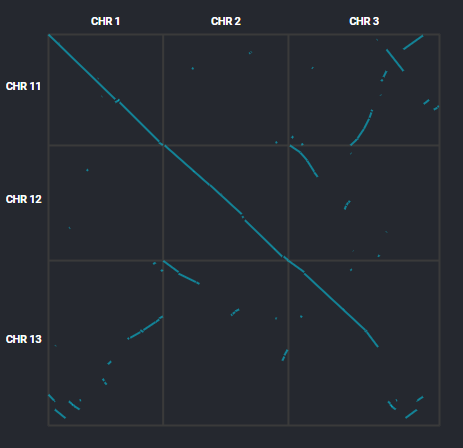
\includegraphics[width=.75\linewidth]{images/ch_1_dot_plot.PNG}
  \captionof{figure}{Dot plot}
  \label{fig:ch_1_dot_plot}
\end{minipage}%
\begin{minipage}{.5\textwidth}
  \centering
  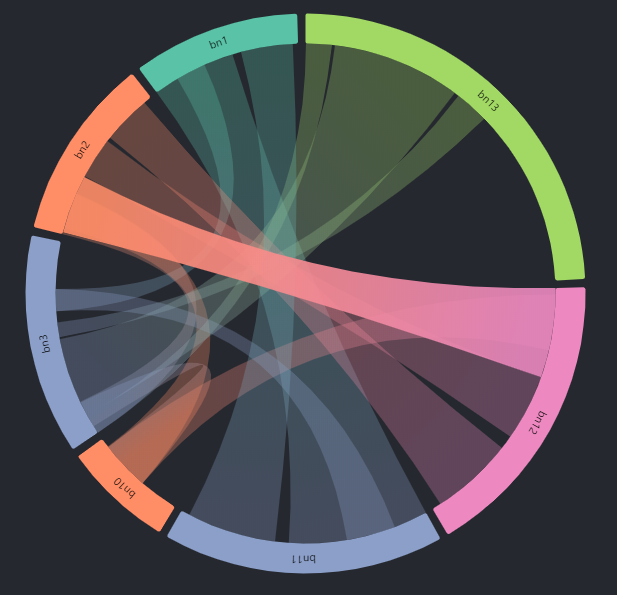
\includegraphics[width=.75\linewidth]{images/ch_1_circos_plot.PNG}
  \captionof{figure}{Circos Plot}
  \label{fig:ch_1_circos_plot}
\end{minipage}
\end{figure}


The sytem should be online and readily avaialble
Generate publication ready high resolution images while still providing small scale images for rapid analysus.








% refernece to https://www.genome.gov/human-genome-project/Completion-FAQ







\section{Problem and Motivation}

The problem addressed in this thesis is that it is difficult to integrated, interactive and easily available

\section{Solution}


\section{Evaluation}

\section{Contribution}

\section{Thesis Outline}